\documentclass[tikz]{standalone}
\usepackage{pgfplots}
\pgfplotsset{compat=1.15}
\usepackage{mathrsfs}
\usetikzlibrary{arrows,calc}
\usepackage{tkz-euclide}
\pagestyle{empty}

\definecolor{AngleClr}{rgb}{0,0.39215686274509803,0}
\definecolor{ShapeClr}{rgb}{0.6,0.2,0}

\begin{document}

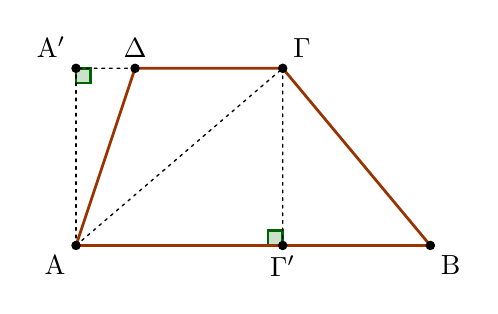
\begin{tikzpicture}[scale=.75]
\tkzSetUpLine[line width=1pt,color=black]
\tkzSetUpPoint[fill=black]

\tkzDefPoints{0/0/A,6/0/B,1/3/D,3.5/3/C}

\tkzDefPointBy[projection=onto C--D](A)\tkzGetPoint{H1}
\tkzDefPointBy[projection=onto A--B](C)\tkzGetPoint{H2}

\tkzFillPolygon[fill=white](A,B,C,D)
\tkzMarkRightAngles[line width=1pt, size=.25,color=AngleClr,fill=AngleClr,fill opacity=0.2](A,H1,C C,H2,A)

\tkzDrawPolygon[color=ShapeClr](A,B,C,D)
\tkzDrawPoints[size=3](A,B,C,D,H1,H2)
\tkzLabelPoint[below left](A){$\rm A$}
\tkzLabelPoint[below right](B){$\rm B$}
\tkzLabelPoint[above right](C){$\rm \Gamma$}
\tkzLabelPoint[above](D){$\rm \Delta$}
\tkzLabelPoint[above left](H1){$\rm A'$}
\tkzLabelPoint[below](H2){$\rm \Gamma'$}

\tkzDrawSegments[line width=0.5pt,color=black,dashed,dash pattern=on 1pt off 1.75pt](A,H1 C,H2 D,H1 A,C)

\end{tikzpicture}
\end{document}
